\section{Double Integrals in Polar Coordinates}\label{sec:DoubleIntegralsinPolarCoordinates}

Suppose we have a surface given in polar coordinates as
$z=f(r,\theta)$ and we wish to find the integral over some region. We
could attempt to translate into rectangular coordinates and do the
integration there, but it is often easier to stay in polar
coordinates.

How might we approximate the volume under such a surface in a way that
uses polar coordinates directly? The basic idea is the same as
before: we divide the region into many small regions, multiply the
area of each small region by the height of the surface somewhere in
that little region, and add them up. What changes is the shape of the
small regions; in order to have a nice representation in terms of $r$
and $\theta$, we use small pieces of ring-shaped areas, as shown in
Figure~\ref{fig:polarcoordinatesregions}. Each small region
is roughly rectangular, except that two sides are segments of a circle
and the other two sides are not quite parallel. Near a point
$(r,\theta)$, the length of either circular arc is about
$r\Delta\theta$ and the length of each straight side is simply $\Delta
r$. When $\Delta r$ and $\Delta \theta$ are very small, the region is
nearly a rectangle with area $r\Delta r\Delta\theta$, and the volume
under the surface is approximately
\[\sum\sum f(r_i,\theta_j)r_i\Delta r\Delta\theta.\]
In the limit, this turns into a double integral
\[\int_{\theta_0}^{\theta_1}\int_{r_0}^{r_1} f(r,\theta)r\,dr\,d\theta.\]

\begin{figure}[H]
\centerline{
\vbox{\beginpicture
\normalgraphs
\setcoordinatesystem units <1.5truecm,1.5truecm>
\setplotarea x from 0 to 4.1, y from 0 to 4.1
\axis left  /
\axis bottom  /
\circulararc 70 degrees from 3.5 0.5 center at 0 0
\circulararc 70 degrees from 2.5 0.5 center at 0 0
\circulararc 60 degrees from 1.5 0.5 center at 0 0
\setlinear
\plot 3.3 1.166 0 0 2.8 2.1 /
\plot 2 2.87 0 0 /
\put {$\Delta r$} [tl] <0pt,-3pt> at 2.9 1
\put {$r\Delta \theta$} [bl] <2pt,2pt> at 3.1 1.62
\endpicture}}
\caption{A polar coordinates ``grid''.}
\label{fig:polarcoordinatesregions}
\end{figure}

\begin{example}{Volume of One-Eighth of a Sphere}{VolumeOneEighthSphere}
Find the volume under $z=\sqrt{4-r^2}$ 
above the quarter circle bounded by
the two axes and the circle $x^2+y^2=4$ in the first quadrant.
\end{example}
\begin{solution}
In terms of $r$ and $\theta$, this region is described by the
restrictions $0\le r\le 2$ and $0\le\theta\le\pi/2$, so we have
\begin{align*}
\int_{0}^{\pi/2}\int_{0}^{2} \sqrt{4-r^2}\;r\,dr\,d\theta
&=\int_{0}^{\pi/2}\left. -{1\over3}(4-r^2)^{3/2}\right|_0^2\,d\theta	\\
&=\int_{0}^{\pi/2} {8\over3}\,d\theta	\\
&={4\pi\over3}.
\end{align*}
The surface is a portion of the sphere of radius 2 centered at the
origin, in fact exactly one-eighth of the sphere. We know the formula
for volume of a sphere is $(4/3)\pi r^3$, so the volume we have
computed is $(1/8)(4/3)\pi 2^3=(4/3)\pi$, in agreement with our
answer.
\end{solution}

This example is much like a simple one in rectangular coordinates: the region
of interest may be described exactly by a constant range for
each of the variables. As with rectangular coordinates, we can adapt
the method to deal with more complicated regions.

\begin{example}{Integration in Polar Coordinates}{integrationinpolarcoordinates}
Find the volume under $z=\sqrt{4-r^2}$ above the region enclosed by the
curve $r=2\cos\theta$, $-\pi/2\le\theta\le\pi/2$; see
Figure~\ref{fig:volumewithvariablelimits}.
\end{example}
\begin{solution}
The region is described in polar coordinates by the inequalities
$-\pi/2\le\theta\le\pi/2$ and $0\le r\le2\cos\theta$, so
the double integral is
\[\int_{-\pi/2}^{\pi/2}\int_{0}^{2\cos\theta} \sqrt{4-r^2}\;r\,dr\,d\theta
=2\int_{0}^{\pi/2}\int_{0}^{2\cos\theta} \sqrt{4-r^2}\;r\,dr\,d\theta.\]
We can rewrite the integral as shown because of the symmetry of the
volume; this avoids a complication during the evaluation.
Proceeding:
\begin{align*}
2\int_{0}^{\pi/2}\int_{0}^{2\cos\theta} \sqrt{4-r^2}\;r\,dr\,d\theta
&=2\int_{0}^{\pi/2}-{1\over3}\left.(4-r^2)^{3/2}\right|_0^{2\cos\theta}\,d\theta	\\
&=2\int_{0}^{\pi/2}-{8\over3}\sin^3\theta+{8\over3}\,d\theta	\\
&=\left.2\left(-{8\over3}{\cos^3\theta\over3}-\cos\theta+{8\over3}\theta\right)\right|_0^{\pi/2}	\\
&={8\over3}\pi-{32\over9}.
\end{align*}
\end{solution}

\begin{figure}[H]
\centerline{
\vbox{\beginpicture
\normalgraphs
\setcoordinatesystem units <1.5truecm,1.5truecm>
\setplotarea x from 0 to 2.1, y from -1.1 to 1.1
\axis left  /
\axis bottom shiftedto y=0 /
\circulararc 360 degrees from 2 0 center at 1 0
\put {\hbox{\epsfxsize6cm\epsfbox{images/polar_volume.eps}}} at 5 0
\endpicture}}
\caption{Volume over a region with non-constant limits.}
\label{fig:volumewithvariablelimits}
\end{figure}

You might have learned a formula for computing areas in polar
coordinates. It is possible to
compute areas as volumes, so that you need only remember one
technique. Consider the surface $z=1$, a horizontal plane. The volume
under this surface and above a region in the $x$-$y$ plane is 
simply $1\cdot(\hbox{area of the region})$, so computing the volume
really just computes the area of the region.

\begin{example}{}{}
Find the area outside the circle $r=2$ and inside
$r=4\sin\theta$; see Figure~\ref{fig:areabyvolume}.
\end{example}
\begin{solution}
The region is described by $\pi/6\le\theta\le5\pi/6$ and
$2\le r\le4\sin\theta$, so the integral is
\begin{align*}
\int_{\pi/6}^{5\pi/6}\int_2^{4\sin\theta}1\,r\,dr\,d\theta
&=\int_{\pi/6}^{5\pi/6}\left. {1\over2}r^2\right|_2^{4\sin\theta}\,d\theta	\\
&=\int_{\pi/6}^{5\pi/6}8\sin^2\theta-2\,d\theta	\\
&={4\over3}\pi+2\sqrt3.
\end{align*}
\end{solution}

\begin{figure}[H]
\centerline{
\hbox{\hfill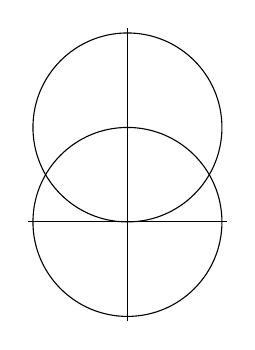
\begin{tikzpicture}[domain=-2:2,x=6mm,y=6mm]
\draw (-2.1,0) -- (2.1,0) ;
\draw (0,-2.1) -- (0,4.1) ;
\draw[color=black] (0,0) circle (2);
\draw[color=black] (0,2) circle (2);
\fill[opacity=0.5,fill=red!20]
plot[parametric,id=first,domain=0.5236:2.618]
function{4*sin(t)*cos(t),4*sin(t)*sin(t)} node {}
plot[parametric,id=second,domain=0.5236:2.618]
function{2*cos(3.1416-t),2*sin(3.1416-t)} -- cycle;
\end{tikzpicture}\hfill}}
\caption{Finding area by computing volume.}
\label{fig:areabyvolume}
\end{figure}


%%%%%%%%%%%%%%%%%%%%%%%%%%%%%%%%%%%%%%%%%%%%
\Opensolutionfile{solutions}[ex]
\section*{Exercises for \ref{sec:DoubleIntegralsinPolarCoordinates}}

\begin{enumialphparenastyle}

\begin{ex}
Find the volume above the $x$-$y$ plane, under the surface
$r^2=2z$, and inside $r=2$.
\begin{sol}
$4\pi$
\end{sol}
\end{ex}

\begin{ex}
Find the volume inside both $r=1$ and $r^2+z^2=4$.
\begin{sol}
$32\pi/3-4\sqrt3\pi$
\end{sol}
\end{ex}

\begin{ex}
Find the volume below $z=\sqrt{1-r^2}$ and above
the top half of the cone $z=r$.
\begin{sol}
$(2-\sqrt2)\pi/3$
\end{sol}
\end{ex}

\begin{ex}
Find the volume below  $z=r$, above the $x$-$y$ plane, and
inside $r=\cos\theta$.
\begin{sol}
$4/9$
\end{sol}
\end{ex}

\begin{ex}
Find the volume below  $z=r$, above the $x$-$y$ plane, and
inside $r=1+\cos\theta$.
\begin{sol}
$5\pi/3$
\end{sol}
\end{ex}

\begin{ex}
Find the volume between $x^2+y^2=z^2$ and $x^2+y^2=z$.
\begin{sol}
$\pi/6$
\end{sol}
\end{ex}

\begin{ex}
Find the area inside $r=1+\sin\theta$ and outside
$r=2\sin\theta$. 
\begin{sol}
$\pi/2$
\end{sol}
\end{ex}

\begin{ex}
Find the area inside both
$r=2\sin\theta$ and $r=2\cos\theta$. 
\begin{sol}
$\pi/2-1$
\end{sol}
\end{ex}

\begin{ex}
Find the area inside the four-leaf rose $r=\cos(2\theta)$
and outside $r=1/2$.
\begin{sol}
$\sqrt3/4+\pi/6$
\end{sol}
\end{ex}

\begin{ex}
Find the area inside the cardioid $r=2(1+\cos\theta)$
and outside $r=2$.
\begin{sol}
$8+\pi$
\end{sol}
\end{ex}

\begin{ex}\label{ex:areaofthreeleafroseloop}
Find the area of one loop of the three-leaf rose
 $r=\cos(3\theta)$.
\begin{sol}
$\pi/12$\
\end{sol}
\end{ex}

\begin{ex}
Compute $\ds \int_{-3}^3\int_0^{\sqrt{9-x^2}}
\sin(x^2+y^2)\,dy\,dx$ by converting to polar coordinates.
\begin{sol}
$(1-\cos(9))\pi/2$
\end{sol}
\end{ex}

\begin{ex}
Compute $\ds \int_{0}^a\int_{-\sqrt{a^2-x^2}}^0 x^2y\,dy\,dx$ 
by converting to polar coordinates.
\begin{sol}
$-a^5/15$
\end{sol}
\end{ex}

\begin{ex}
Find the volume under $z=y^2+x+2$ above
the region $x^2+y^2\le 4$
\begin{sol}
$12\pi$
\end{sol}
\end{ex}

\begin{ex}
Find the volume between
$z=x^2y^3$ and $z=1$ above
the region $x^2+y^2\le 1$
\begin{sol}
$\pi$
\end{sol}
\end{ex}

\begin{ex}
Find the volume inside
$x^2+y^2=1$ and $x^2+z^2=1$.
\begin{sol}
$16/3$
\end{sol}
\end{ex}

\begin{ex}
Find the volume under $z=r$ above $r=3+\cos\theta$.
\begin{sol}
$21\pi$
\end{sol}
\end{ex}

\begin{ex}
Figure~\ref{fig:doubleflower} shows the plot of
$r=1+4\sin(5\theta)$.
\begin{figure}[H]
\centerline{
\vbox{\beginpicture
\normalgraphs
\setcoordinatesystem units <2truecm,2truecm>
\setplotarea x from -1 to 1, y from -1 to 1
\put {\hbox{\epsfxsize4cm\epsfbox{images/double_flower.eps}}} at 0 0
\endpicture}}
\caption{$r=1+4\sin(5\theta)$}
\label{fig:doubleflower}
\end{figure}
\begin{enumerate}
	\item Describe the behavior of the graph in terms of the given
	  equation.  Specifically, explain maximum and minimum values, number
	  of leaves, and the 'leaves within leaves'.
	\item Give an integral or integrals to determine the area outside a
	  smaller leaf but inside a larger leaf.
	\item How would changing the value of $a$ in the equation
	  $r=1+a\cos(5\theta)$ change the relative sizes of the inner and
	  outer leaves? Focus on values $a\geq 1$.  (Hint: How would we change
	  the maximum and minimum values?)
\end{enumerate}
\end{ex}

\begin{ex}
Consider the integral $\ds\iint_D {1\over\sqrt{x^2+y^2}} \;
dA$, where $D$ is the unit disk centered at the origin.
\begin{enumerate}
	\item Why might this integral be considered improper?
	\item Calculate the value of the integral of the same function
	  $\ds 1/\sqrt{x^2+y^2}$ over the annulus with outer radius 1 and
	  inner radius $\delta$.
	\item Obtain a value for the integral on the whole disk by letting
	  $\delta$ approach 0.
		\begin{sol}
		$2\pi$
		\end{sol}
	\item For which values $\lambda$ can we replace the denominator with
	  $(x^2+y^2)^\lambda$ in the original integral?
\end{enumerate}
\end{ex}

\end{enumialphparenastyle}